\chapter{Results}
%Figure \ref{fig:cpd_perf}, shows accuracy and detection time as a function of the
%false positive rate per second, for the OSU Hip dataset,
%for each of the SVM, Decision Tree, and Neural Net base classifiers.
%
%\begin{figure}
% \centering
% \includegraphics[scale=0.3]{osu_cpd_dt_acc.png}
% \includegraphics[scale=0.3]{osu_cpd_svm_acc.png}
% \includegraphics[scale=0.3]{osu_cpd_nnet_acc.png}
% \includegraphics[scale=0.3]{osu_cpd_dt_det.png}
% \includegraphics[scale=0.3]{osu_cpd_svm_det.png}
% 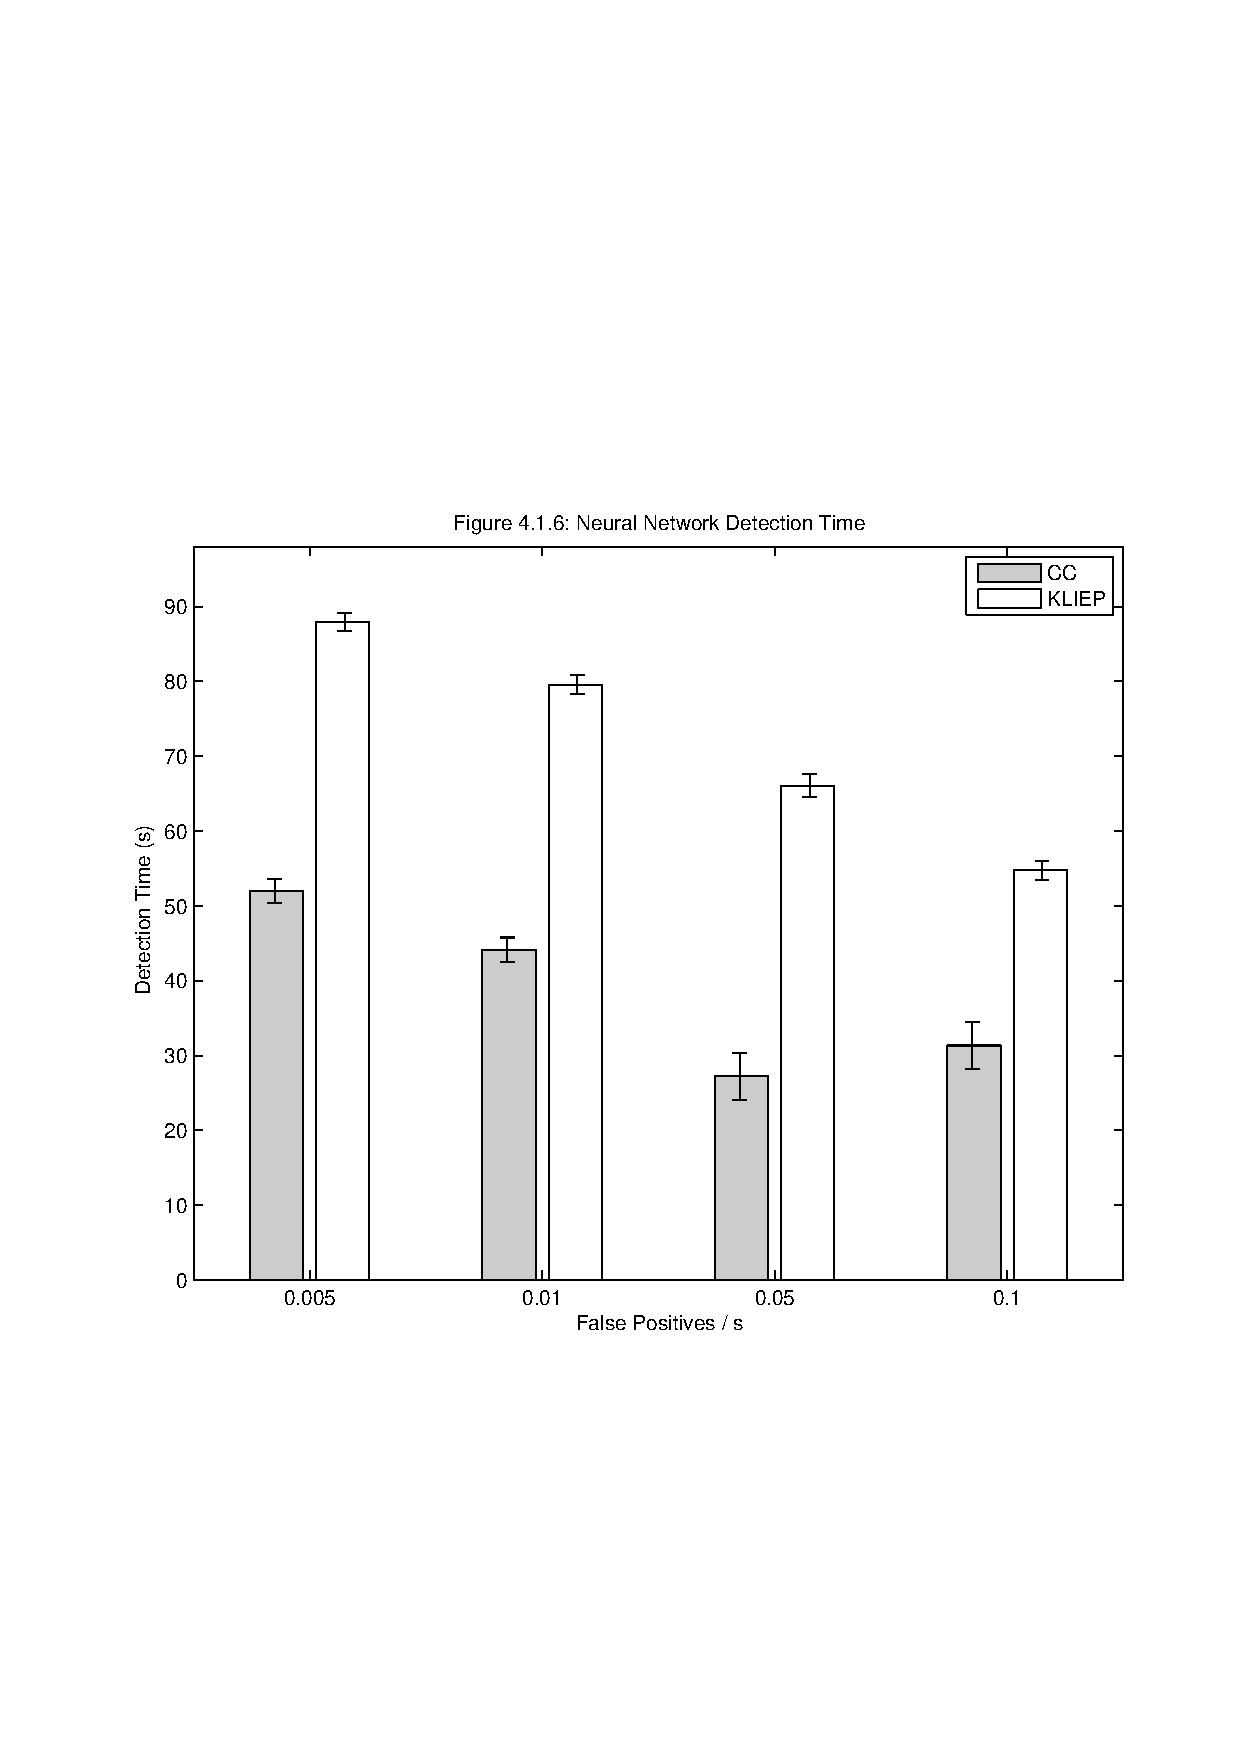
\includegraphics[scale=0.3]{osu_cpd_nnet_det.png}
% \caption{CPD-Based Classification Performance}
% \label{fig:cpd_perf}
%\end{figure}

\section{Change-Point Detection}
\label{sec:cpd_results}

Results for our change-point detection experiments are given in
Figures \ref{fig:osu_cpd}-\ref{fig:lime2_cpd}.
The performance of the change-point detection algorithms
depended heavily on the threshold level for change prediction. In our
experiment we varied the threshold level, thus changing the false positive
rate. A large number of false positives per
second were tested, but for the sake of brevity only a representative sample
of $\{0.005, 0.01, 0.05, 0.1\}$ are shown here.

In the OSU Hip experiments, control charts outperformed KLIEP in terms of
detection time (Figures 4.1.2, 4.1.4, 4.1.6), while the accuracy results 
(Figures 4.1.1, 4.1.3, 4.1.5) were
mixed. Except when predicted windows are large enough to span across multiple
true activities, it is generally expected that accuracy will decrease as false
positive rate increases because small windows contain less information and are
less discriminative than larger windows. This behavior is seen in the control chart
accuracy results (grey bars in Figures 4.1.1, 4.1.3, 4.1.5), but not in the
KLIEP accuracy results (white bars in Figures 4.1.1, 4.1.3, 4.1.5).
Follow-up experiments showed that KLIEP peaks in accuracy for
false positives per second between $0.2$ and $0.3$ for all three classifiers.
KlIEP seemed to perform best on this dataset when it was given many
opportunities to predict changes.

Further investigation indicated that across the OSU Hip dataset the KLIEP algorithm
was unable to detect many of the different activity changes without a very low score
threshold value (and a very high false positive rates).
Some qualitative plotting of the OSU Hip data showed
that most of its activities have accelerometer amplitude values that strongly
resemble draws from a multivariate normal distribution. Since control charts
assume that the data is drawn from a distribution that is a member of that
family, it is logical that control charts would outperform algorithms with
different modeling assumptions on OSU Hip.

In the LiME experiments, KLIEP outperformed control charts in terms of
accuracy across the board, and control charts outperformed KLIEP in terms of
detection time across the board. This suggests that in general control charts
correctly detected true changes more quickly, but that after a correct change
prediction it was more likely to make an incorrect change prediction.

In a few cases (Figures 4.1.2, 4.1.6, 4.2.6) the detection time did
not decrease as the false positive rate increased. On the face of it this would seem
to be a non-sequitur, but this only happened in cases when accuracy also decreased
(Figures 4.1.1, 4.1.5, 4.2.5).
Smaller window sizes tend to be correlated with decreased detection times, but
it is possible that predicting with smaller windows, if they happen to contain
an insufficient amount of discriminative data,
can actually increase the time required for the classifier to start correctly
predicting the ground-truth activity. Additionally, the given increases in detection
time were small and within confidence bounds.

\begin{figure}[H]
 \includegraphics[scale=0.4]{osu_cpd_dt_acc.pdf} \hspace{1em}\vspace{1em}
 \includegraphics[scale=0.4]{osu_cpd_dt_det.pdf}
 \includegraphics[scale=0.4]{osu_cpd_svm_acc.pdf} \hspace{1em}\vspace{1em}
 \includegraphics[scale=0.4]{osu_cpd_svm_det.pdf}
 \includegraphics[scale=0.4]{osu_cpd_nnet_acc.pdf} \hspace{2em}
 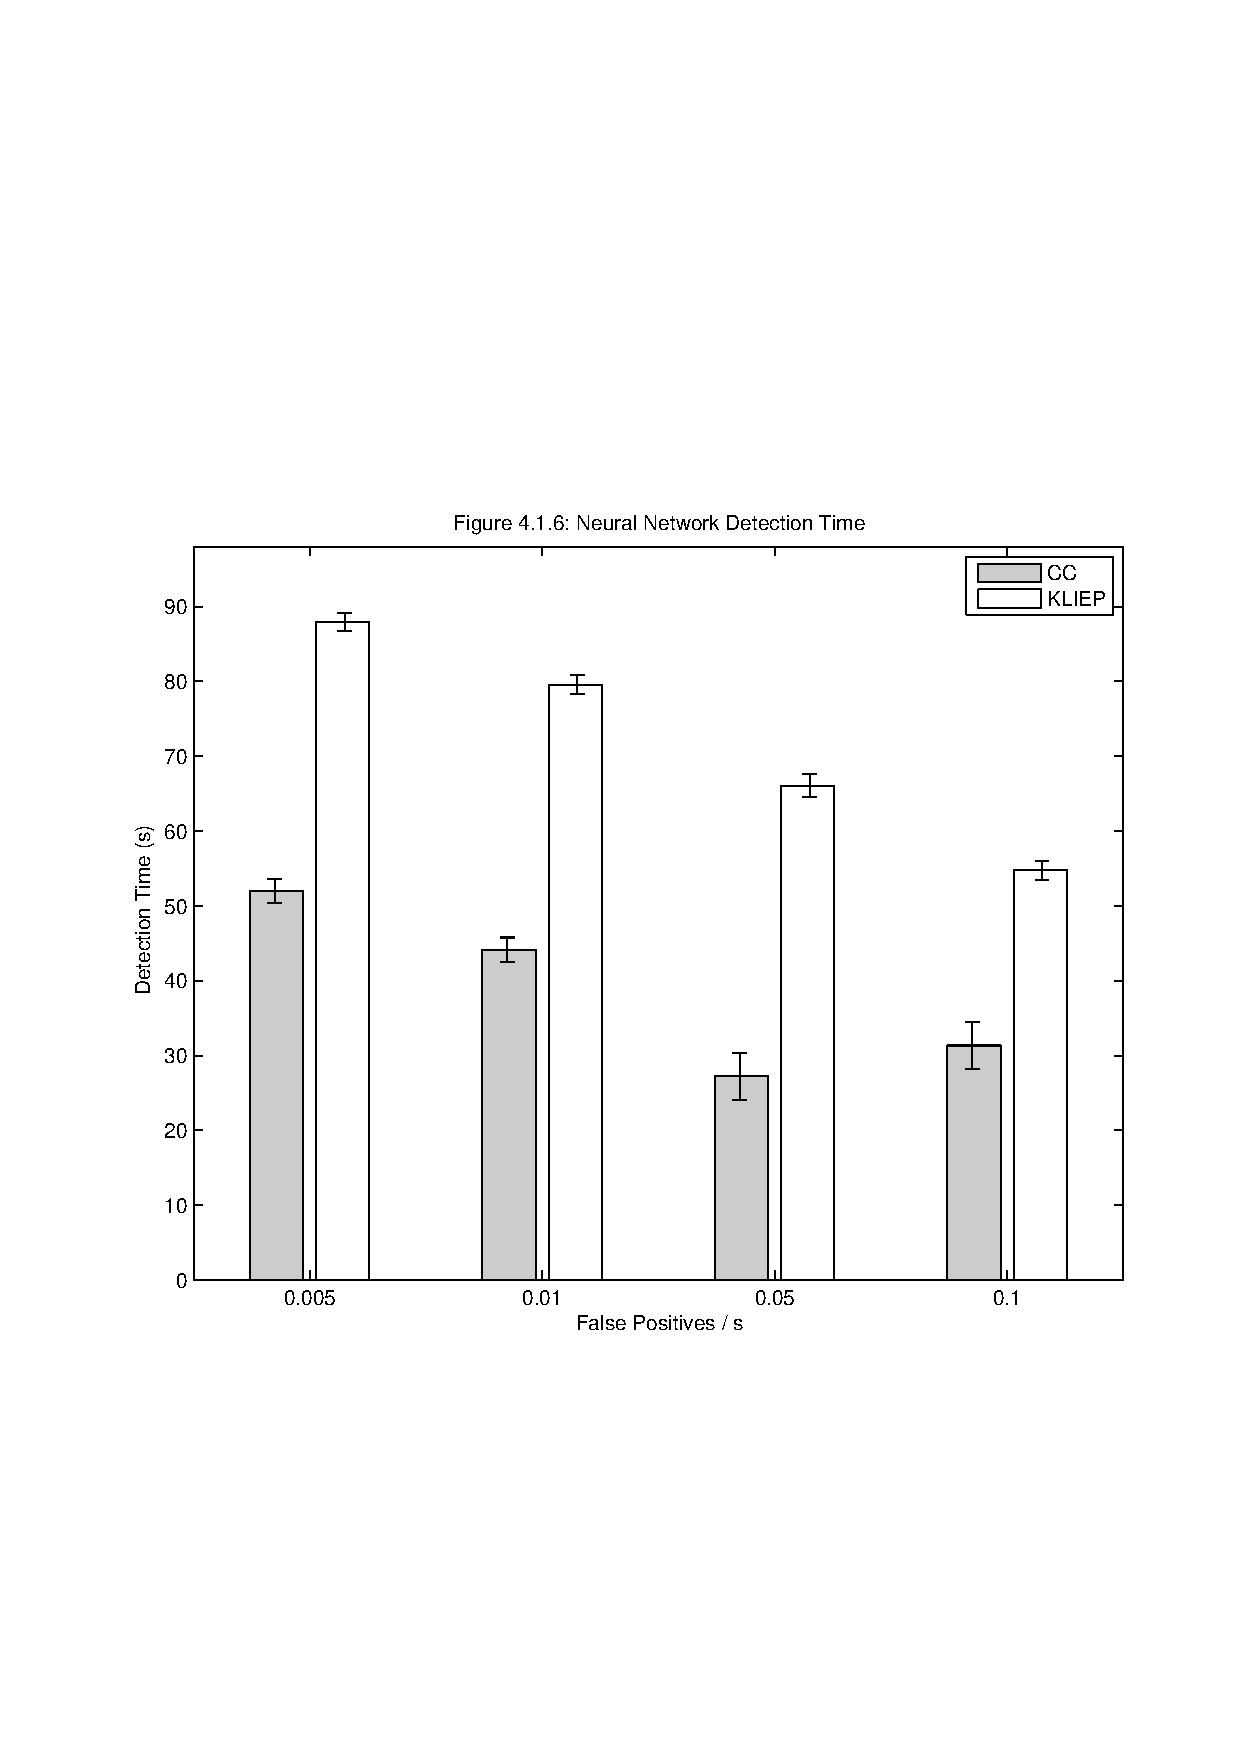
\includegraphics[scale=0.4]{osu_cpd_nnet_det.pdf}
 \caption{OSU Hip Results. Graphs are organized into rows by base classifier,
  and columns by evaluation metric. Change-point detection results were averaged over
  30 splits into training, testing, and validation datasets. Error bars show a
  95\% confidence interval around the average.}
 \label{fig:osu_cpd}
\end{figure}

\begin{figure}[H]
 \centering
 \includegraphics[scale=0.4]{lime1_cpd_dt_acc.pdf} \hspace{1em}\vspace{1em}
 \includegraphics[scale=0.4]{lime1_cpd_dt_det.pdf}
 \includegraphics[scale=0.4]{lime1_cpd_svm_acc.pdf} \hspace{1em}\vspace{1em}
 \includegraphics[scale=0.4]{lime1_cpd_svm_det.pdf}
 \includegraphics[scale=0.4]{lime1_cpd_nnet_acc.pdf} \hspace{1em}
 \includegraphics[scale=0.4]{lime1_cpd_nnet_det.pdf}
 \caption{LiME Day 1 Results. Graphs are organized into rows by base classifier,
  and columns by evaluation metric. Change-point detection results were averaged over
  30 splits into training, testing, and validation datasets. Error bars show a
  95\% confidence interval around the average.}
 \label{fig:lime1_cpd}
\end{figure}

\begin{figure}[H]
 \centering
 \includegraphics[scale=0.4]{lime2_cpd_dt_acc.pdf} \hspace{1em}\vspace{1em}
 \includegraphics[scale=0.4]{lime2_cpd_dt_det.pdf}
 \includegraphics[scale=0.4]{lime2_cpd_svm_acc.pdf} \hspace{1em}\vspace{1em}
 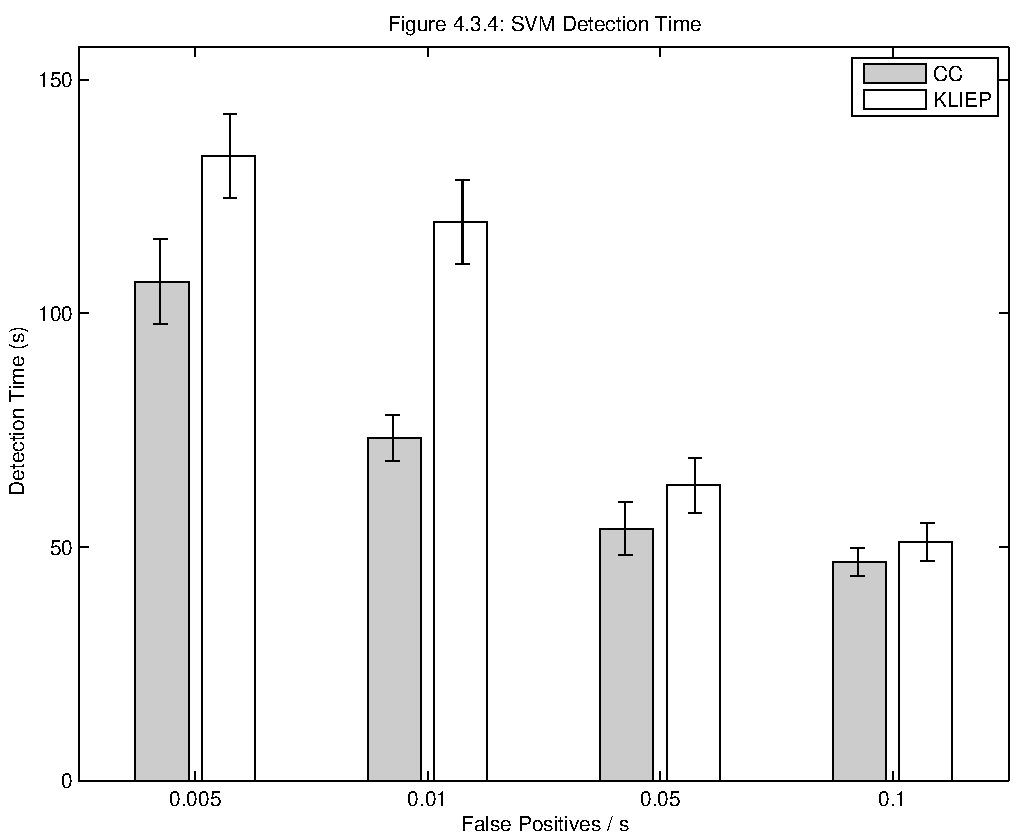
\includegraphics[scale=0.4]{lime2_cpd_svm_det.pdf}
 \includegraphics[scale=0.4]{lime2_cpd_nnet_acc.pdf} \hspace{1em}
 \includegraphics[scale=0.4]{lime2_cpd_nnet_det.pdf}
 \caption{LiME Day 2 Results. Graphs are organized into rows by base classifier,
  and columns by evaluation metric. Change-point detection results were averaged over
  30 splits into training, testing, and validation datasets. Error bars show a
  95\% confidence interval around the average.}
 \label{fig:lime2_cpd}
\end{figure}


\section{HMM}

Results for our HMM experiments are given in
Figures \ref{fig:osu_hmm}-\ref{fig:lime2_hmm}. Each HMM experiment was
performed by splitting each time series into windows of fixed length
corresponding to discrete time ``ticks'' in an HMM,
and results for windows of length $\{10, 12, 14, 16, 18, 20\}$
seconds are shown.

For all three base classifiers, accuracy was high and
stable with respect to window size, over all three datasets. Detection
time was also fairly stable in the OSU Hip experiments, though as would
generally be expected it increased somewhat with window size in the LiME
experiments. Further experiments [results not shown] on the
OSU Hip dataset showed that the accuracy and detection time of our HMM approach 
tends to be poor for very small window sizes, but that it stabilizes with window sizes
that are greater than roughly 5 seconds. This gives a strong indication that
5 seconds is the amount of information necessary for the classifiers to become as
discriminative as they can be on the datasets in our work.
 
\begin{figure}[H]
 \centering
 \includegraphics[scale=0.4]{osu_hmm_dt_acc.pdf} \hspace{1em}\vspace{1em}
 \includegraphics[scale=0.4]{osu_hmm_dt_det.pdf}
 \includegraphics[scale=0.4]{osu_hmm_svm_acc.pdf} \hspace{1em}\vspace{1em}
 \includegraphics[scale=0.4]{osu_hmm_svm_det.pdf}
 \includegraphics[scale=0.4]{osu_hmm_nnet_acc.pdf} \hspace{1em}
 \includegraphics[scale=0.4]{osu_hmm_nnet_det.pdf}
 \caption{OSU Hip HMM Results.
  Graphs are organized into rows by base classifier, and columns by evaluation
  metric. HMM results were averaged over 10 splits into training
  (base classifier), validation, training (HMM), and testing datasets. Error
  bars show a 95\% confidence interval around the average.}
 \label{fig:osu_hmm}
\end{figure}

\begin{figure}[H]
 \centering
 \includegraphics[scale=0.4]{lime1_hmm_dt_acc.pdf} \hspace{1em}\vspace{1em}
 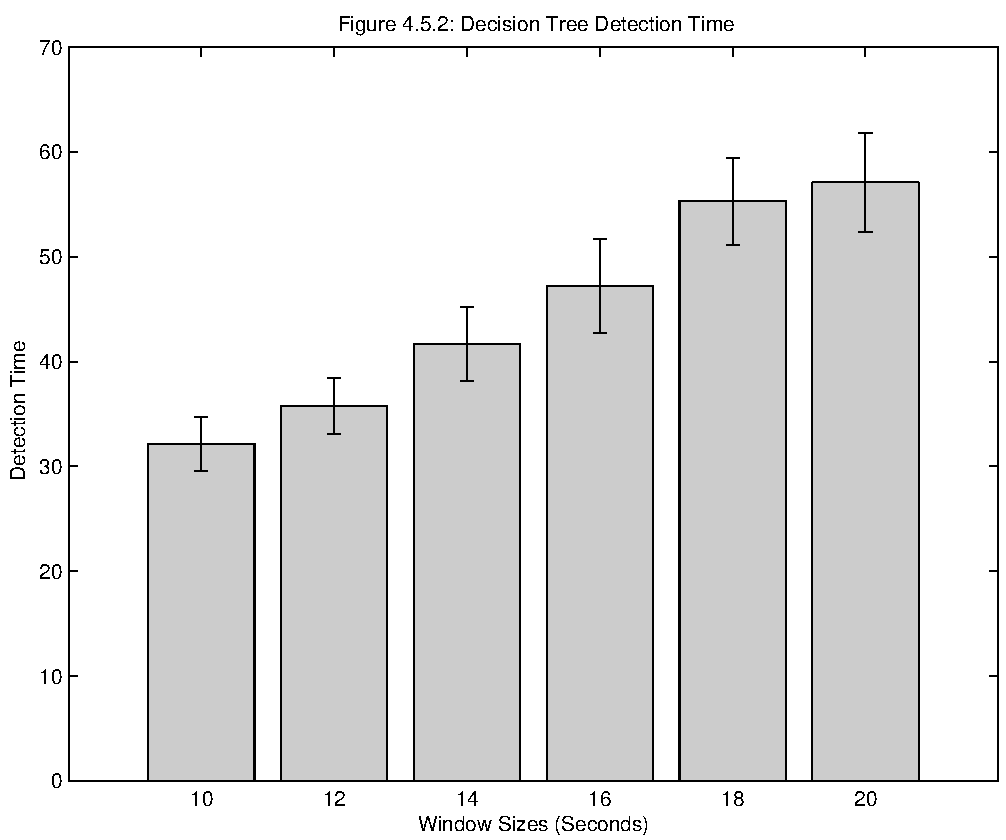
\includegraphics[scale=0.4]{lime1_hmm_dt_det.pdf} 
 \includegraphics[scale=0.4]{lime1_hmm_svm_acc.pdf} \hspace{1em}\vspace{1em}
 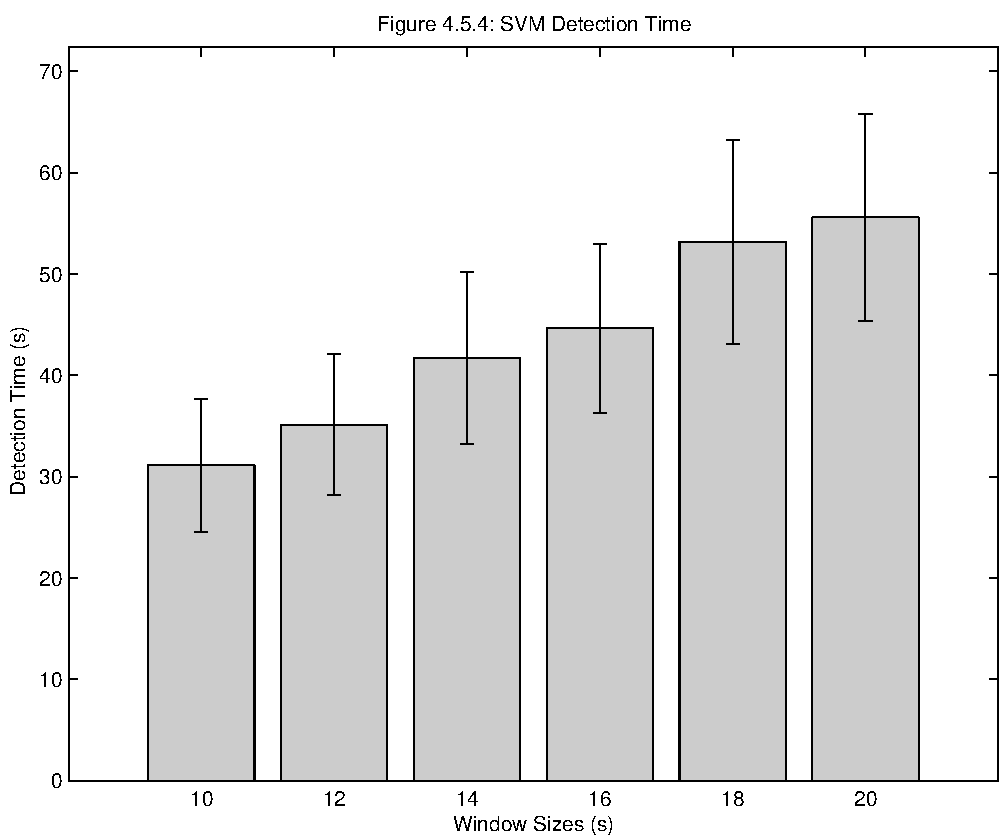
\includegraphics[scale=0.4]{lime1_hmm_svm_det.pdf} 
 \includegraphics[scale=0.4]{lime1_hmm_nnet_acc.pdf} \hspace{1em}
 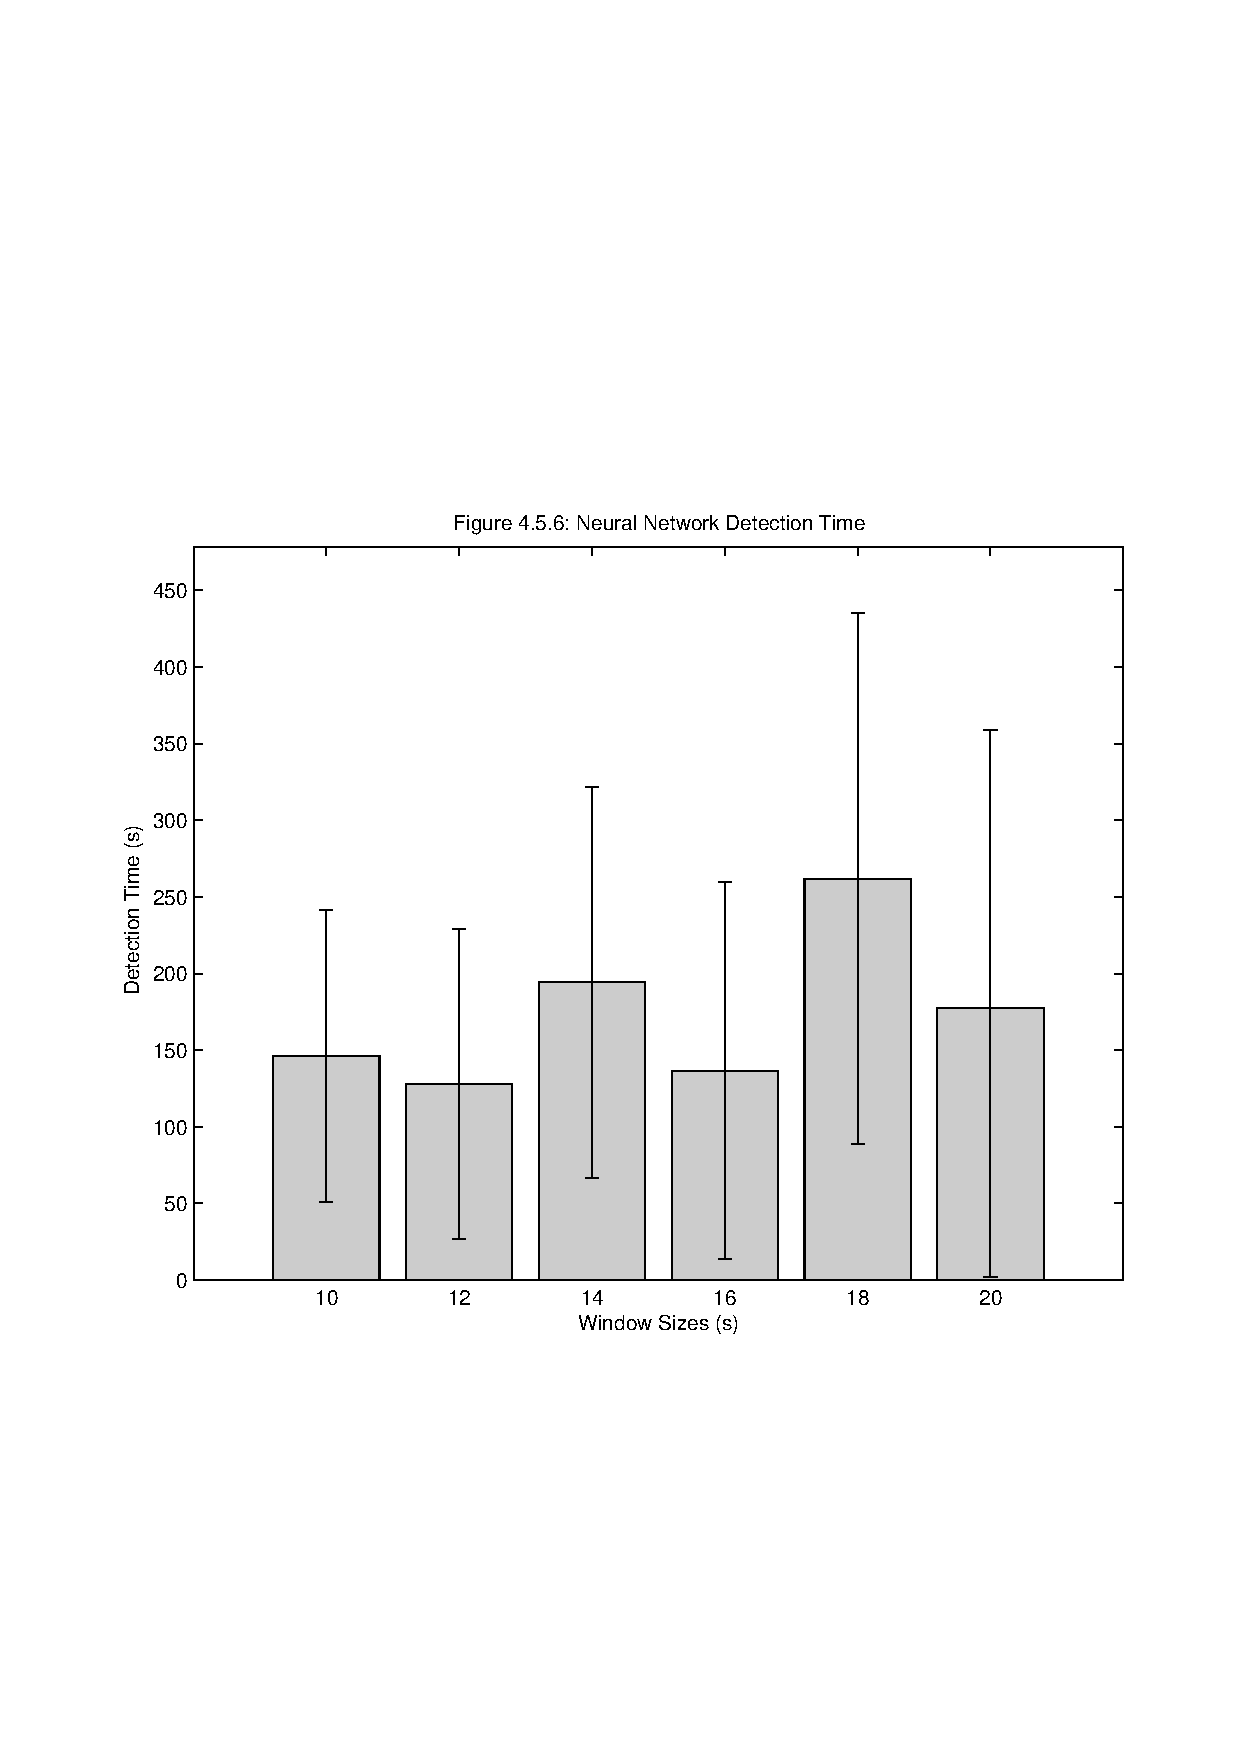
\includegraphics[scale=0.4]{lime1_hmm_nnet_det.pdf} 
 \caption{LiME Day 1 HMM Results.
  Graphs are organized into rows by base classifier, and columns by evaluation
  metric. HMM results were averaged over 10 splits into training
  (base classifier), validation, training (HMM), and testing datasets. Error
  bars show a 95\% confidence interval around the average.}
 \label{fig:lime1_hmm}
\end{figure}

\begin{figure}[H]
 \centering
 \includegraphics[scale=0.4]{lime2_hmm_dt_acc.pdf} \hspace{1em}\vspace{1em}
 \includegraphics[scale=0.4]{lime2_hmm_dt_det.pdf}
 \includegraphics[scale=0.4]{lime2_hmm_svm_acc.pdf} \hspace{1em}\vspace{1em}
 \includegraphics[scale=0.4]{lime2_hmm_svm_det.pdf}
 \includegraphics[scale=0.4]{lime2_hmm_nnet_acc.pdf} \hspace{1em}
 \includegraphics[scale=0.4]{lime2_hmm_nnet_det.pdf}
 \caption{LiME Day 2 HMM Results.
  Graphs are organized into rows by base classifier, and columns by evaluation
  metric. HMM results were averaged over 10 splits into training
  (base classifier), validation, training (HMM), and testing datasets. Error
  bars show a 95\% confidence interval around the average.}
 \label{fig:lime2_hmm}
\end{figure}

\newpage

\section{Discussion}

We found it difficult to directly compare the performance between the change-
point detection and HMM approaches, because we
varied false positives per second in the change-point detection experiments,
and varied the fixed-length window size in the HMM experiments.
However, for a given false positive rate change-point
detection algorithms split a time series into windows of a certain average size,
which generally decreases as the false positive rate increases. From this it is possible
to relate false positive rates from the change-point detection experiments to
the window sizes of the HMM experiments. HMM false positive rates per second of
\{0.033, 0.028, 0.024, 0.021, 0.019, 0.017\} correspond to average
window sizes of \{10, 12, 14, 16, 18, 20\}. Figures \ref{fig:osu_compare_cpd_hmm},
\ref{fig:lime1_compare_cpd_hmm}, and \ref{fig:lime2_compare_cpd_hmm}
show a side-by-side comparison of the top-down and bottom-up approaches, using
this conversion. As seen in Section \ref{sec:cpd_results}, two algorithms 
were tested for each of the change-point detection experiments, but only the
best performing algorithm (highest in accuracy or lowest in detection time) is 
shown here, for each individual experiment.
Our results show that the HMM approach outperformed the change-point
detection approach, both in terms of accuracy
and detection time, regardless of the dataset and base classifier.

The experiments so far shown did not isolate the reason for the difference in
performance between the top-down and bottom-up approaches. Further
experimentation was necessary to determine if the difference was caused by the
use of change-point detection algorithms to segment the data as opposed to using
fixed length windows, or if the difference was caused by the ability of the HMM
to smooth predictions made on temporal data. A side-by-side comparison of the
same fixed window length classification experiments performed with and without HMM smoothing
(see Figures \ref{fig:osu_compare_nohmm}, \ref{fig:lime1_compare_nohmm}, and
\ref{fig:lime2_compare_nohmm}) suggested that the smoothing effect of the HMM
did not explain most of the performance difference, and that the performance difference between the top-down
and bottom-up approaches was mostly due to noisy segmentation by the change-point
detection algorithms.

Nonetheless, a contributing factor to the particularly high accuracy and low detection time
results generally attained for the OSU Hip experiments was that the data
consisted of activities that were synthetically glued together. The same group
of activities were performed in the same order by each of the 50 subjects in
this dataset, making transitions from one activity to the other very predictable
for a temporal model. By contrast, the LiME datasets consisted of unsynthetic
data gathered from a large set of unstructured and variable-length activities,
so the activity transitions were not as predictable and are more indicative of
an application of our techniques in the real world.

A final point of interest was that SVM (Figures 4.7.3, 4.7.4, 4.8.3, 4.8.4, 4.9.3, 4.9.4) clearly outperformed the other two
base classifiers, and that the faster and simpler decision tree model (Figures 4.7.1, 4.7.2, 4.8.1, 4.8.2, 4.9.1, 4.9.2) matched up
well against neural networks (Figures 4.7.5, 4.7.6, 4.8.5, 4.8.6, 4.9.5, 4.9.6). This result is significant because much of the
previous research that has formulated activity detection as a supervised learning
problem has used neural networks exclusively.

\begin{figure}[h]
 \centering
 %\includegraphics[scale=0.3]{vspace.png}
 \includegraphics[scale=0.4]{osu_dt_cpd_hmm_compare_acc_line.pdf} \hspace{1em}\vspace{1em}
 \includegraphics[scale=0.4]{osu_dt_cpd_hmm_compare_det_line.pdf} 
 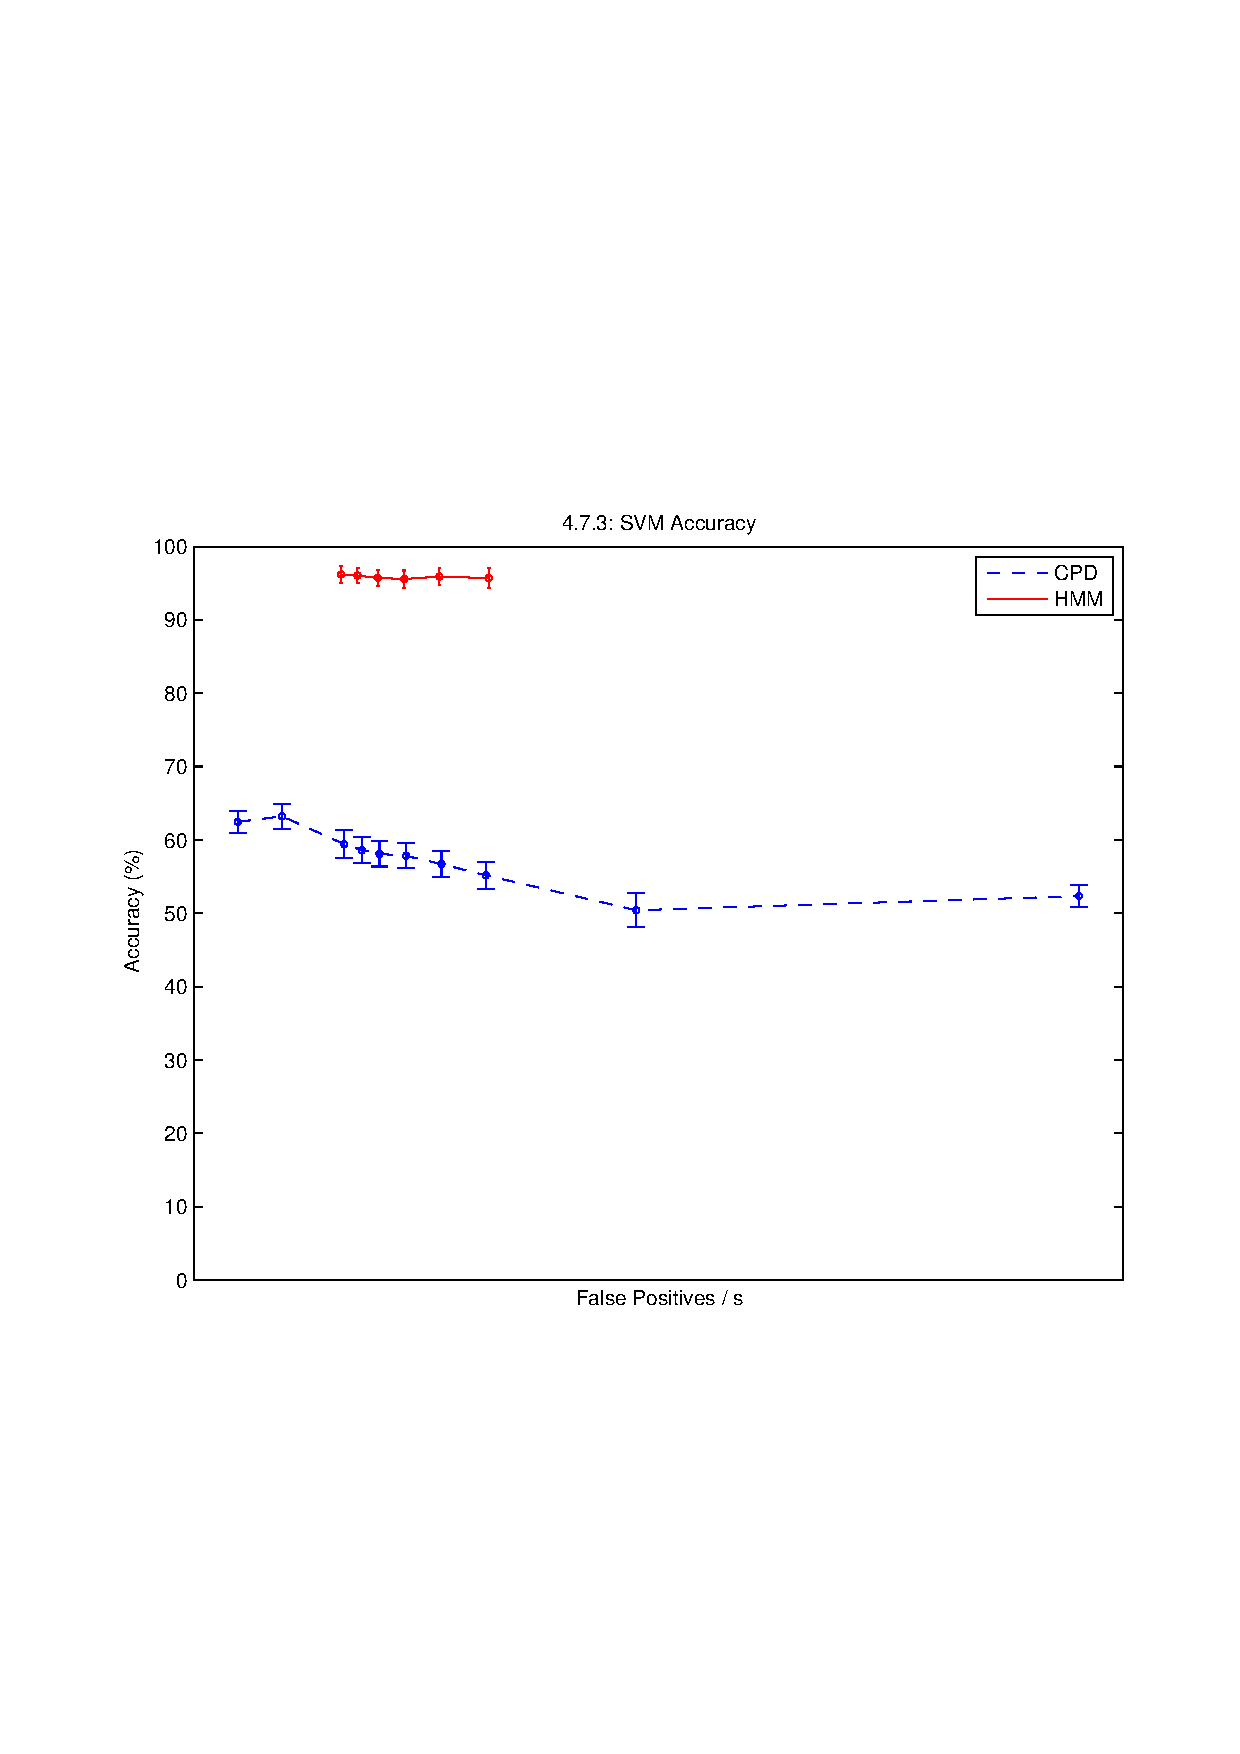
\includegraphics[scale=0.4]{osu_svm_cpd_hmm_compare_acc_line.pdf} \hspace{1em}\vspace{1em}
 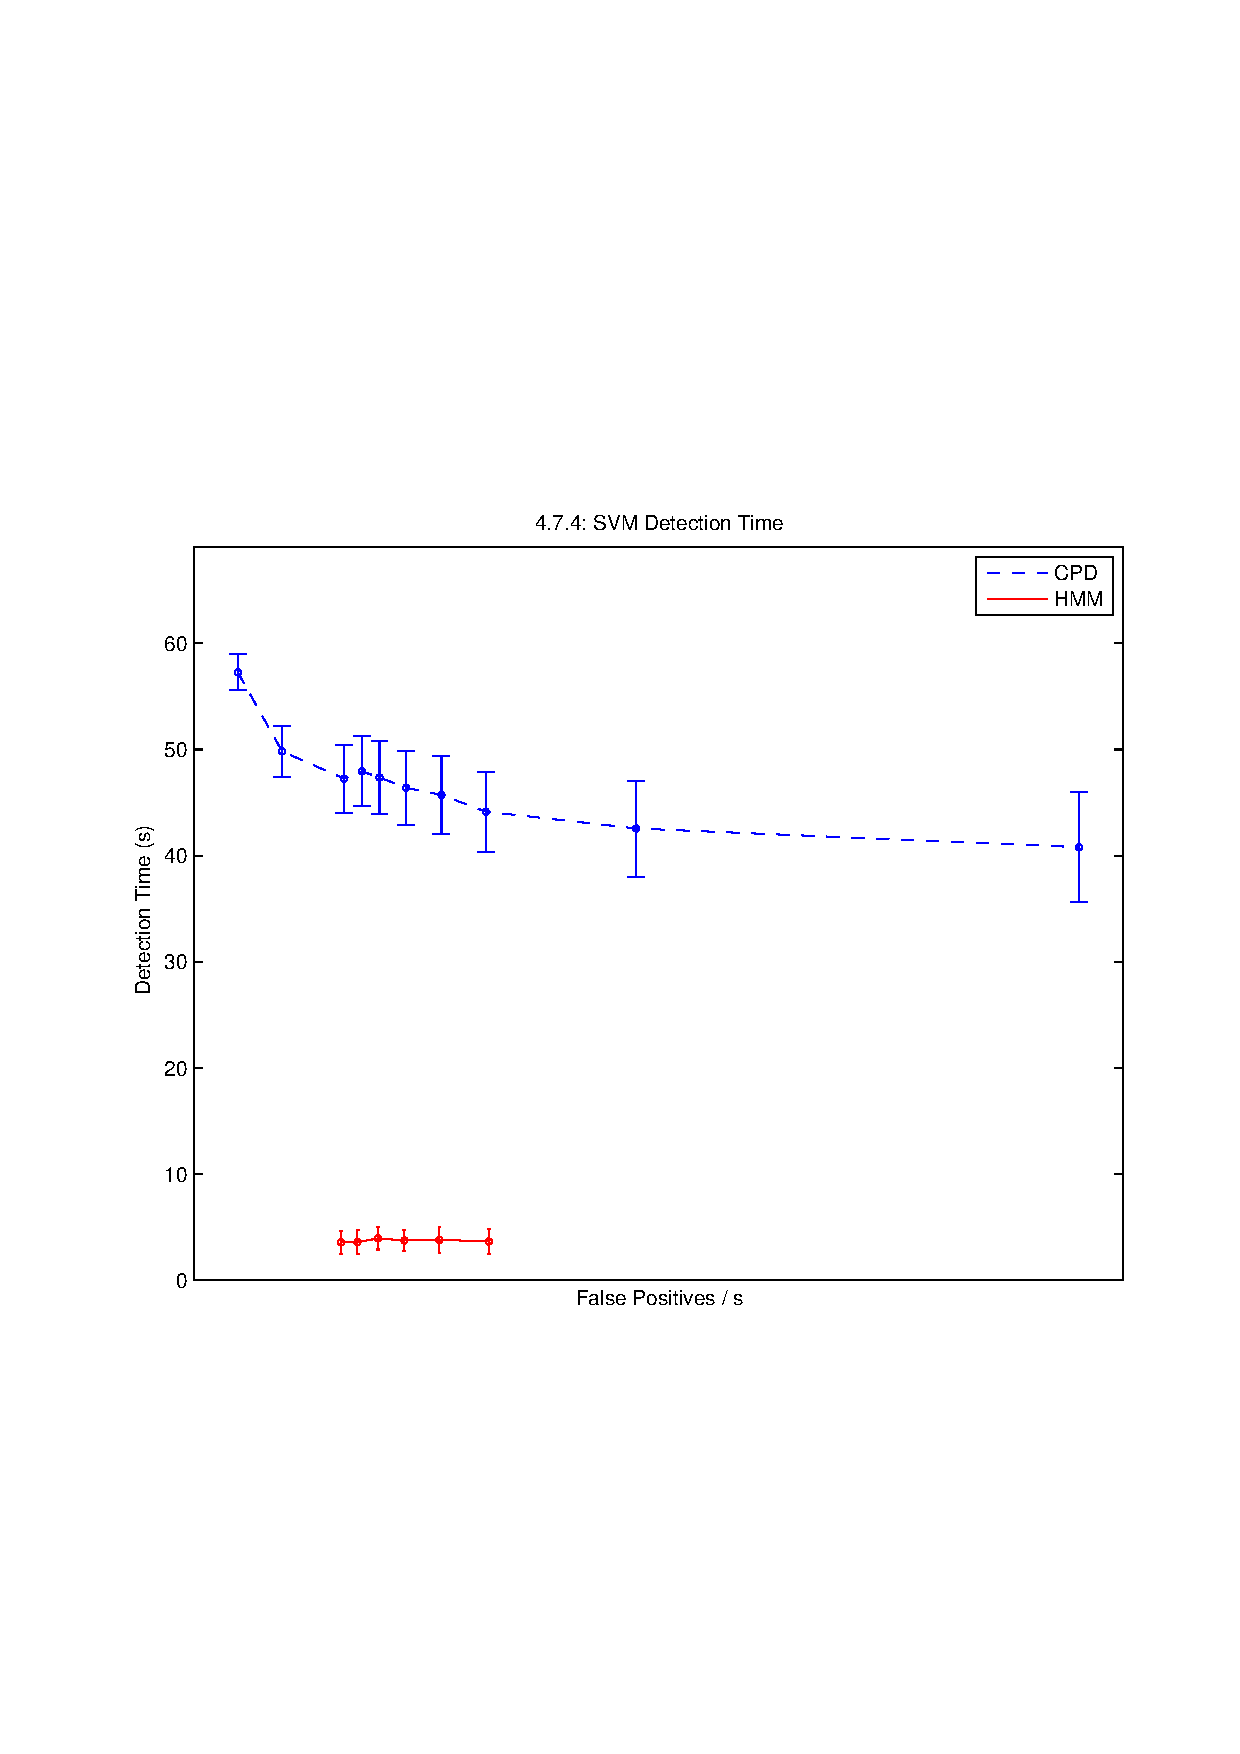
\includegraphics[scale=0.4]{osu_svm_cpd_hmm_compare_det_line.pdf}
 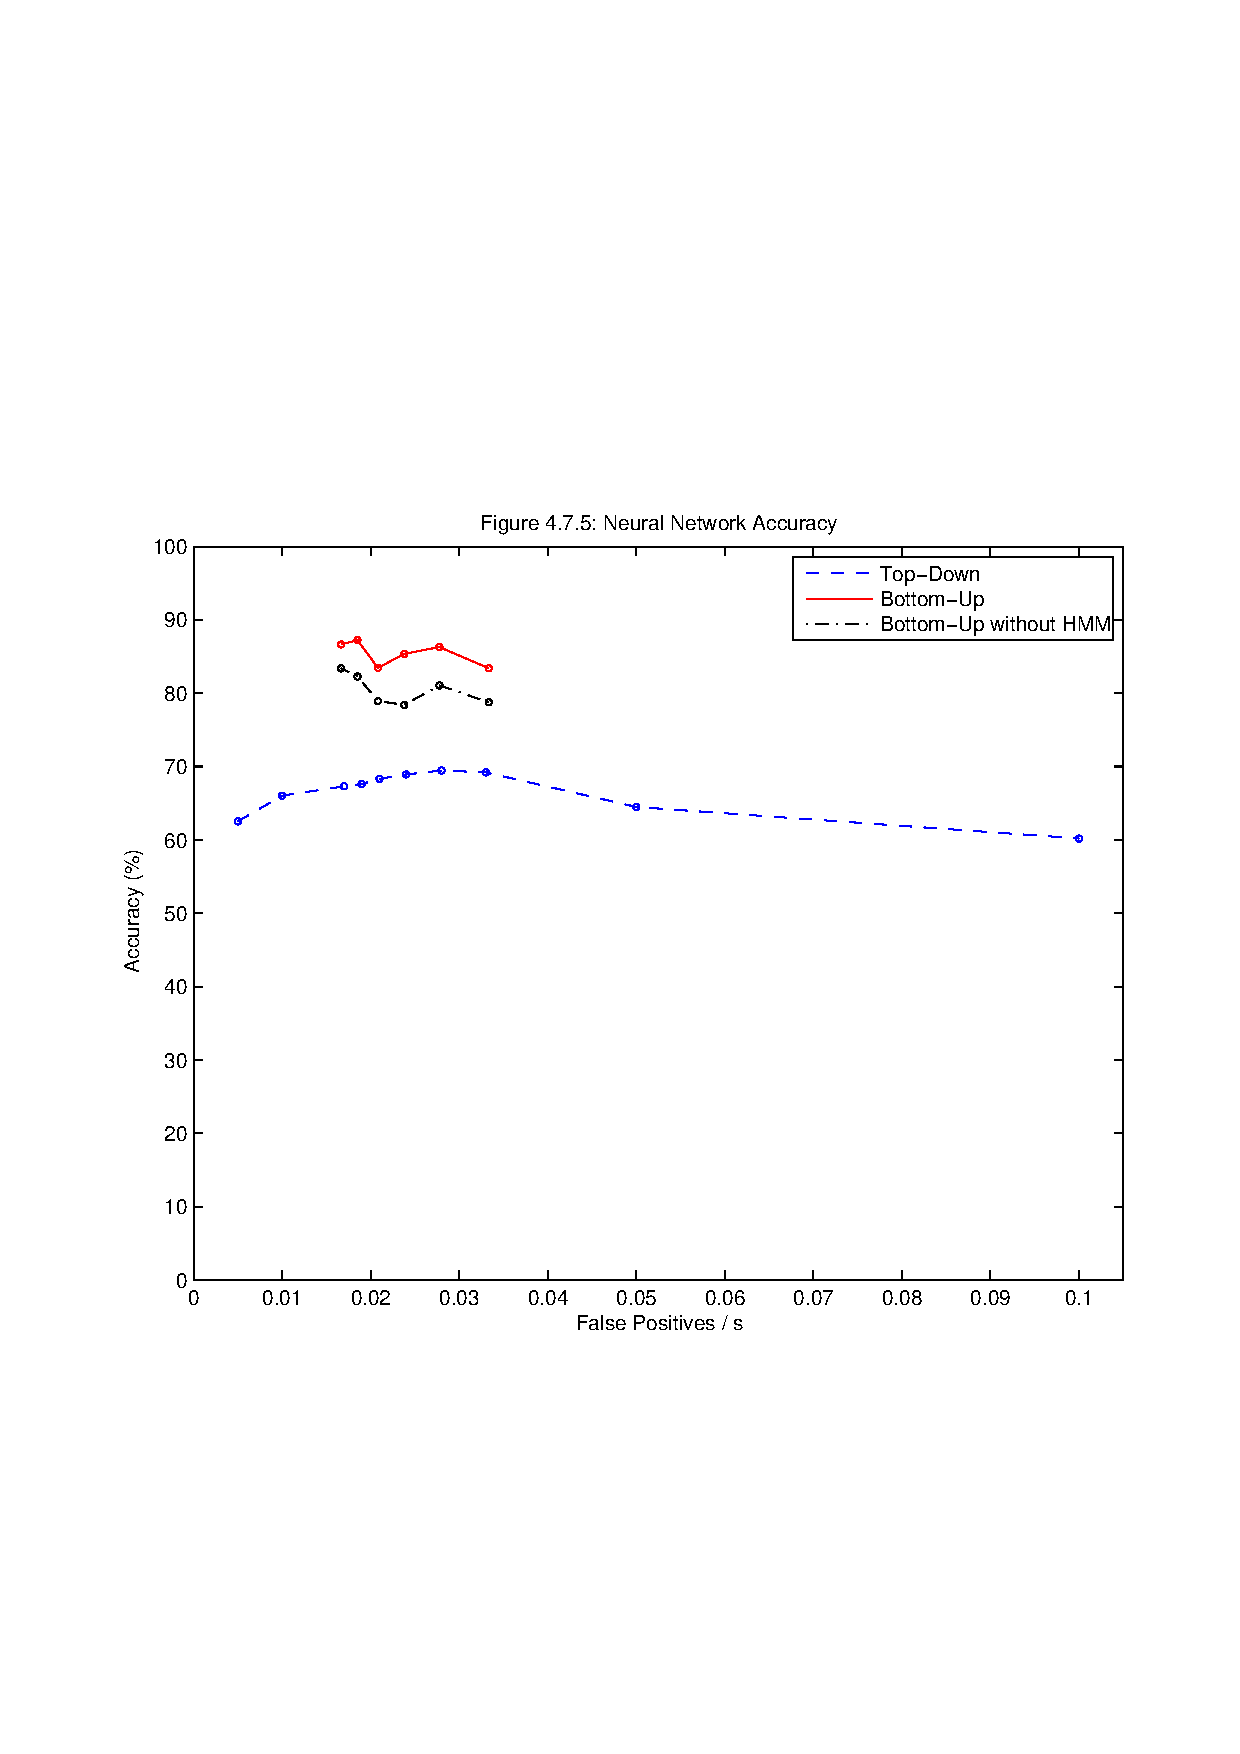
\includegraphics[scale=0.4]{osu_nnet_cpd_hmm_compare_acc_line.pdf} \hspace{1em}
 \includegraphics[scale=0.4]{osu_nnet_cpd_hmm_compare_det_line.pdf}
 \caption{Comparison of change-point detection and HMM results for OSU Hip.
  Graphs are organized into rows by base classifier, and columns by evaluation
  metric. Results for false positives per second of \{0.005, 0.01, 0.05, 0.1\} are change-point
  detection experiments, while results for false positives per second of
  \{0.017, 0.019, 0.021, 0.024, 0.028, 0.033\} are HMM experiments. Error bars
  show a 95\% confidence interval.}
 \label{fig:osu_compare_cpd_hmm}
\end{figure}

\begin{figure}[h]
 \centering
 %\includegraphics[scale=0.3]{vspace.png}
 \includegraphics[scale=0.4]{lime1_dt_cpd_hmm_compare_acc_line.pdf} \hspace{1em}\vspace{1em}
 \includegraphics[scale=0.4]{lime1_dt_cpd_hmm_compare_det_line.pdf} 
 \includegraphics[scale=0.4]{lime1_svm_cpd_hmm_compare_acc_line.pdf} \hspace{1em}\vspace{1em}
 \includegraphics[scale=0.4]{lime1_svm_cpd_hmm_compare_det_line.pdf}
 \includegraphics[scale=0.4]{lime1_nnet_cpd_hmm_compare_acc_line.pdf} \hspace{1em}
 \includegraphics[scale=0.4]{lime1_nnet_cpd_hmm_compare_det_line.pdf}
 \caption{Comparison of change-point detection and HMM results for LiME Day 1.
  Graphs are organized into rows by base classifier, and columns by evaluation
  metric. Results for false positives per second of \{0.005, 0.01, 0.05, 0.1\} are change-point
  detection experiments, while results for false positives per second of
  \{0.017, 0.019, 0.021, 0.024, 0.028, 0.033\} are HMM experiments. Error bars
  show a 95\% confidence interval.}
 \label{fig:lime1_compare_cpd_hmm}
\end{figure}

\begin{figure}[h]
 \centering
 %\includegraphics[scale=0.3]{vspace.png}
 \includegraphics[scale=0.4]{lime2_dt_cpd_hmm_compare_acc_line.pdf} \hspace{1em}\vspace{1em}
 \includegraphics[scale=0.4]{lime2_dt_cpd_hmm_compare_det_line.pdf} 
 \includegraphics[scale=0.4]{lime2_svm_cpd_hmm_compare_acc_line.pdf} \hspace{1em}\vspace{1em}
 \includegraphics[scale=0.4]{lime2_svm_cpd_hmm_compare_det_line.pdf}
 \includegraphics[scale=0.4]{lime2_nnet_cpd_hmm_compare_acc_line.pdf} \hspace{1em}
 \includegraphics[scale=0.4]{lime2_nnet_cpd_hmm_compare_det_line.pdf}
 \caption{Comparison of change-point detection and HMM results for LiME Day 2.
  Graphs are organized into rows by base classifier, and columns by evaluation
  metric. Results for false positives per second of \{0.005, 0.01, 0.05, 0.1\} are change-point
  detection experiments, while results for false positives per second of
  \{0.017, 0.019, 0.021, 0.024, 0.028, 0.033\} are HMM experiments. Error bars
  show a 95\% confidence interval.}
 \label{fig:lime2_compare_cpd_hmm}
\end{figure}


\begin{figure}[h]
 \centering
 %\includegraphics[scale=0.3]{vspace.png}
 \includegraphics[scale=0.4]{osu_dt_hmm_nohmm_compare_acc.pdf} \hspace{1em}\vspace{1em}
 \includegraphics[scale=0.4]{osu_dt_hmm_nohmm_compare_det.pdf} 
 \includegraphics[scale=0.4]{osu_svm_hmm_nohmm_compare_acc.pdf} \hspace{1em}\vspace{1em}
 \includegraphics[scale=0.4]{osu_svm_hmm_nohmm_compare_det.pdf}
 \includegraphics[scale=0.4]{osu_nnet_hmm_nohmm_compare_acc.pdf} \hspace{1em}
 \includegraphics[scale=0.4]{osu_nnet_hmm_nohmm_compare_det.pdf}
 \caption{Comparison of base classifier performance with and without HMM
  smoothing layer, with test data split into fixed window sizes. Graphs are organized into rows by base
  classifier, and columns by evaluation metric. Error bars show a 95\% confidence interval.}
 \label{fig:osu_compare_nohmm}
\end{figure}

\begin{figure}[h]
 \centering
 %\includegraphics[scale=0.3]{vspace.png}
 \includegraphics[scale=0.4]{lime1_dt_hmm_nohmm_compare_acc.pdf} \hspace{1em}\vspace{1em}
 \includegraphics[scale=0.4]{lime1_dt_hmm_nohmm_compare_det.pdf} 
 \includegraphics[scale=0.4]{lime1_svm_hmm_nohmm_compare_acc.pdf} \hspace{1em}\vspace{1em}
 \includegraphics[scale=0.4]{lime1_svm_hmm_nohmm_compare_det.pdf}
 \includegraphics[scale=0.4]{lime1_nnet_hmm_nohmm_compare_acc.pdf} \hspace{1em}
 \includegraphics[scale=0.4]{lime1_nnet_hmm_nohmm_compare_det.pdf}
 \caption{Comparison of base classifier performance with and without HMM
  smoothing layer, with test data split into fixed window sizes. Graphs are organized into rows by base
  classifier, and columns by evaluation metric. Error bars show a 95\% confidence interval.}
 \label{fig:lime1_compare_nohmm}
\end{figure}

\begin{figure}[h]
 \centering
 %\includegraphics[scale=0.3]{vspace.png}
 \includegraphics[scale=0.4]{lime2_dt_hmm_nohmm_compare_acc.pdf} \hspace{1em}\vspace{1em}
 \includegraphics[scale=0.4]{lime2_dt_hmm_nohmm_compare_det.pdf} 
 \includegraphics[scale=0.4]{lime2_svm_hmm_nohmm_compare_acc.pdf} \hspace{1em}\vspace{1em}
 \includegraphics[scale=0.4]{lime2_svm_hmm_nohmm_compare_det.pdf}
 \includegraphics[scale=0.4]{lime2_nnet_hmm_nohmm_compare_acc.pdf} \hspace{1em}
 \includegraphics[scale=0.4]{lime2_nnet_hmm_nohmm_compare_det.pdf}
 \caption{Comparison of base classifier performance with and without HMM
  smoothing layer, with test data split into fixed window sizes. Graphs are organized into rows by base
  classifier, and columns by evaluation metric. Error bars show a 95\% confidence interval.}
 \label{fig:lime2_compare_nohmm}
\end{figure}

\section{Timing}

Since we are interested in the feasibility of performing activity detection on
accelerometer data in real time, we tested how long it would require our
approaches to segment and classify a time series in a streaming, online fashion.
Experiments were performed using an Intel(R) Core(TM) 2 Quad Processor Q9550.

There are three different computations that a device must perform to do
activity recognition in real time. The first (when using the top-down approach)
is to calculate a change-point
detection score for an individual time tick. When the device obtains a new tick of
accelerometer data, it must generate a change-point detection score and compare
it to the score threshold to decide whether or not to predict an activity
change. We estimated the amount of time required to determine whether an
activity change should be predicted by choosing 1000 random ticks from our data,
and running our two change-point detection algorithms on the reference and test
data corresponding to each tick. We found that on average the control chart algorithm
took 0.050ms per tick, and that the KLIEP algorithm took 31.4ms per tick. If no change
was predicted, then the device needs to take no further action for this tick.

If a change was predicted in the first step, then the second step is to
featurize the window of data corresponding to the activity that just ended.
The amount of time required to featurize an activity window increases with the
length of the window. The OSU Hip dataset contained 120 second long activities,
and the median length of the LiME activities was considerably smaller than that,
therefore we fixed the window length at 120 seconds for this experiment. The
amount of time required to featurize these windows, again averaged over 1000 runs,
was 98.5ms.

Once the data from an activity window is featurized, the activity must be
predicted using a base classifier. We assume that the classifier has already
been trained and validated previously. We averaged the activity prediction time
over 60 runs on each of our base classifiers, with featurized windows and models
built during our change-point detection experiments. We found that the average
time required to predict an activity with decision trees was 372ms, with
SVMs was 368ms, and with neural networks was 369ms.

These experiments show that the amount of time required to process an activity
tick when a change is predicted is in the worst case
31.4ms + 98.5ms + 372ms = 501ms, which is a very reasonable amount of time
for an online application.
